\scanpage{321}
\[
\diagram{\begin{tikzcd}
X\arrow[r,"\text{degré }n"]&Y\\
\Gamma^n(X)\arrow[ur]&{}
\end{tikzcd}}
\qquad F(X)\overset{?}{\unsure{-|\longrightarrow}}F(Y)
\]
\deleted{
\[
\diagram{\begin{tikzcd}
F(\Gamma^nX)\arrow[r,no head]&F(Y)\\
\Gamma^n(F(X))\arrow[u]\arrow[ur]&{}
\end{tikzcd}}
\]
\figure{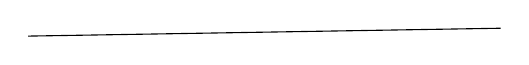
\begin{tikzpicture}\draw(0,0)--(6,.1);\end{tikzpicture}}
\[
F_A(X)=\operatorname{Hom}_A(X)
\]
\[
\diagram{\begin{tikzcd}
\Gamma^nF_A(X)\arrow[r,"?"]&F_A(\Gamma^nX)
\end{tikzcd}}
\]
\[
\diagram{\begin{tikzcd}
\Gamma^n\operatorname{Hom}_1(A,X)\arrow[r,"\unsure{\beta}?"]&\operatorname{Hom}_1(A,\Gamma^nX)
\end{tikzcd}}
\]
\deleted{$\unsure{\beta(u^{(n)})}\longrightarrow\unsure{A}\cdot\Gamma^n(f)$}
\unsure{foncteur} en $\unsure{A|X}$
\[
\unsure{Y|X}\longrightarrow X\otimes X
\]
\margin{bilin, \unsure{fonct.} en $X,Y$}
\[
\diagram{\begin{tikzcd}
F_{\unsure{C|A}}(X\otimes Y)&F_A(X)\times F_{\unsure{B|A}}(Y)\arrow[l]
\end{tikzcd}}
\]
\inserted{$\unsure{\varphi}$}
: si $X=Y=A$, l’image $\mathrm{id}_A,\mathrm{id}_A$ donne un élt
\[
A\longrightarrow A\otimes A
\]
\unsure{comparer}

a) associativité : \unsure{associativité} de la coalg.

b) \uline{commutativité}

c) compatible avec $1$ i.e.
\[
\diagram{\begin{tikzcd}
\unsure{k_\varphi|h_\varphi}\arrow[r]&F_A(1)=\\
{}&\operatorname{Hom}(A,1)\arrow[u,equals]
\end{tikzcd}}
\]
\unsure{re.}\quad\unsure{coaugm}\quad $A\overset{u}{\longrightarrow}1$
\figure{
\begin{tikzpicture}\draw (0,0)--(1.5,.06);\end{tikzpicture}}
}
\figure{\begin{tikzpicture}\draw(0,8)--(4,0);\end{tikzpicture}}
\margin{322}
